\subsection{The  future directions of gesture-based UI}

In summary, Gesture-based user interfaces will stay relevant and push us today on how we interact with our own devices. From the explosion of the Internet of things and the drop of unit price on camera sensors areas such as the Cars Industry, Public transport, Medical Research, and the Games Industry will see large exciting advancements in the field. From my analysis gesture recognition systems are dependent on how technology advanced the region's society is. As reported by Grand View Research  ' China and India are among the fastest-growing economies in the world,  Increasing disposable income and growing industrial digitization are poised to supplement the growth of the region.' This proves true by the Gantt chart created as shown in Fig 6.1.



It is for certain the complexity and speed of devices are allowing for the addition of gestures but the market is preventing mainstream use of gestures of classical hardware. Gesture recognition is a reasonably new technology and needs further testing in areas such as Medicine, Teaching automobiles only trial and error can tell its stability. Due to the COVID-19 pandemic as of early 2019, we have been faced with new ways of interacting. In my opinion gesture technologies will prevail as we try to reduce the physical contact with our devices to prevent bacteria on our devices.



 \begin{figure}[h!]
  \centering
    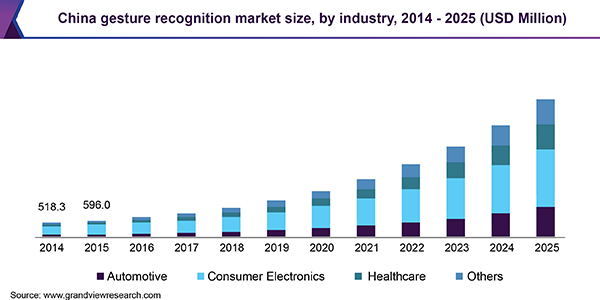
\includegraphics[width=0.7\textwidth]{Research-Latex/images/futureOfGestures.png}
     \caption{China's explosion in gesture popularity}
\end{figure}